% ===========================================================================
%  03 — 系统架构
%
%  声明: C-ARCH-01, C-ARCH-02, C-ARCH-03, C-PROC-01, C-PROC-02,
%        C-TELEM-01, C-RAG-01, C-VLM-01, C-VLM-02, C-RUNTIME-01
% ===========================================================================
\chapter{系统架构}\label{ch:system-design}

本章从架构层面回答RQ1：如何将模拟器遥测、检索到的过程性知识以及视觉观测整合在一起，使得教学输出保持状态感知、可审计且对过程性引导安全？核心设计决策是将基础模型的输出视为证据约束运行时中的一个阶段，而非教学者本身。每一条帮助响应都由显式证据包生成，对照过程包规则进行检查，由校验器验证，通过覆盖层白名单映射，并记录以供回放。

本章首先从证据锚定问题出发推导设计需求。随后介绍端口-适配器架构、实时帮助循环、遥测与过程门控证据层、校验器验证机制、模拟器适配器边界、日志与回放基础设施，以及VLM衍生视觉事实的运行时角色。数据集构建与VLM微调方法论留待第~\ref{ch:methodology}~章讨论；实现层面的细节见第~\ref{ch:implementation}~章。

% ===========================================================================
\section{设计需求}\label{sec:design-goals}

基于证据的过程性教学对系统提出了与传统清单式应用或不受约束的LLM聊天机器人截然不同的需求。运行时必须观测状态、根据过程顺序进行推理、以语言解释帮助内容，同时防止未经支持的覆盖层操作到达学习者。以下六项需求指导架构设计。

\begin{itemize}
\item \textbf{G1 -- 实时过程状态观测。}
教学者必须通过模拟器状态（而非仅靠学习者自述）来观测学习者的进度。在F/A-18C场景中，这意味着在有结构化数据导出的地方使用DCS-BIOS遥测，在座舱显示状态未以结构化数据形式导出的地方使用视觉事实。

\item \textbf{G2 -- 过程感知的步骤推断。}
教学者必须基于前置条件、完成门控和序列历史进行推理。下一个有用的帮助条目不一定是清单上的下一行，而是在当前证据下有效的下一个操作。

\item \textbf{G3 -- 可操作输出的显式证据。}
每一个推荐的步骤、覆盖层目标或拒绝推进的决定都必须可追溯到证据：遥测数据、门控结果、检索到的过程性来源、最近的状态变化或视觉事实。仅凭模型流畅的语言输出不足以作为证据。

\item \textbf{G4 -- 清晰的架构边界。}
领域逻辑必须独立于模拟器API、模型提供方、GPU可用性以及VR显示管道。这使得核心过程逻辑和验证逻辑可以在没有运行中模拟器的情况下进行测试。

\item \textbf{G5 -- 优雅降级。}
当模型输出不可用、格式错误或证据锚定不足时，运行时必须回退到确定性文本引导或安全拒绝，而非执行不安全的覆盖层操作。

\item \textbf{G6 -- 声明式过程配置。}
过程步骤、门控、遥测映射、UI目标、视觉事实绑定以及错误分类标准必须表示为一个过程包，而非隐藏在提示词或适配器代码中。这使得任务模型可检查且可版本控制。
\end{itemize}

这些需求解释了为什么系统被设计为证据管线。该架构并不试图让语言模型本身足够可靠以独立行动，而是用显式状态证据、声明式规则、Schema验证、白名单和可回放日志来包围模型的生成过程。

% ===========================================================================
\section{端口-适配器架构}\label{sec:design-arch}

运行时遵循端口-适配器架构，依赖方向严格：外部系统通过适配器连接，适配器实现稳定的端口，核心层包含过程逻辑和验证逻辑。核心层绝不导入DCS特定、提供方特定或VR特定的模块。这一边界对论文的核心论点至关重要，因为证据锚定必须能够在脱离实时模拟器的条件下进行测试和检查。

\begin{description}
\item[核心层 (Core layer).]
核心层包含与模拟器无关的领域逻辑：过程状态追踪、门控评估、视觉事实状态合并、BM25检索原语、事件类型、响应Schema生成、证据包构造、校验器验证、评分以及面向回放的状态检查。

\item[端口层 (Ports layer).]
端口层定义领域核心与外部世界之间的稳定接口。主要端口涵盖模型推理、知识检索、视觉输入和遥测输入。这些端口使得替换模型提供方、知识后端或模拟器适配器时无需修改过程引擎。

\item[适配器层 (Adapters layer).]
适配器层包含外部集成代码：DCS-BIOS接收器、遥测数据清洗与聚合、DCS覆盖层分发、OpenAI兼容及本地模型客户端、BM25文档检索、截图捕获以及VLM视觉事实提取。

\item[过程包 (Procedure packs).]
过程包是核心层消费的任务特定契约。F/A-18C过程包定义了步骤顺序、前置门控、完成门控、UI目标标识符、遥测变量映射、视觉事实绑定以及错误分类标准。它不是适配器，因为它不与模拟器通信；它是声明式的领域规格说明。
\end{description}

图~\ref{fig:system-architecture}~总结了该架构。该图应从左到右解读为一条证据流：模拟器状态与座舱图像通过适配器进入，过程包规则构建运行时的解释框架，检索到的来源与模型服务支持帮助生成，校验器在输出到达座舱之前检查生成的操作计划。

\begin{figure}[htbp]
  \centering
  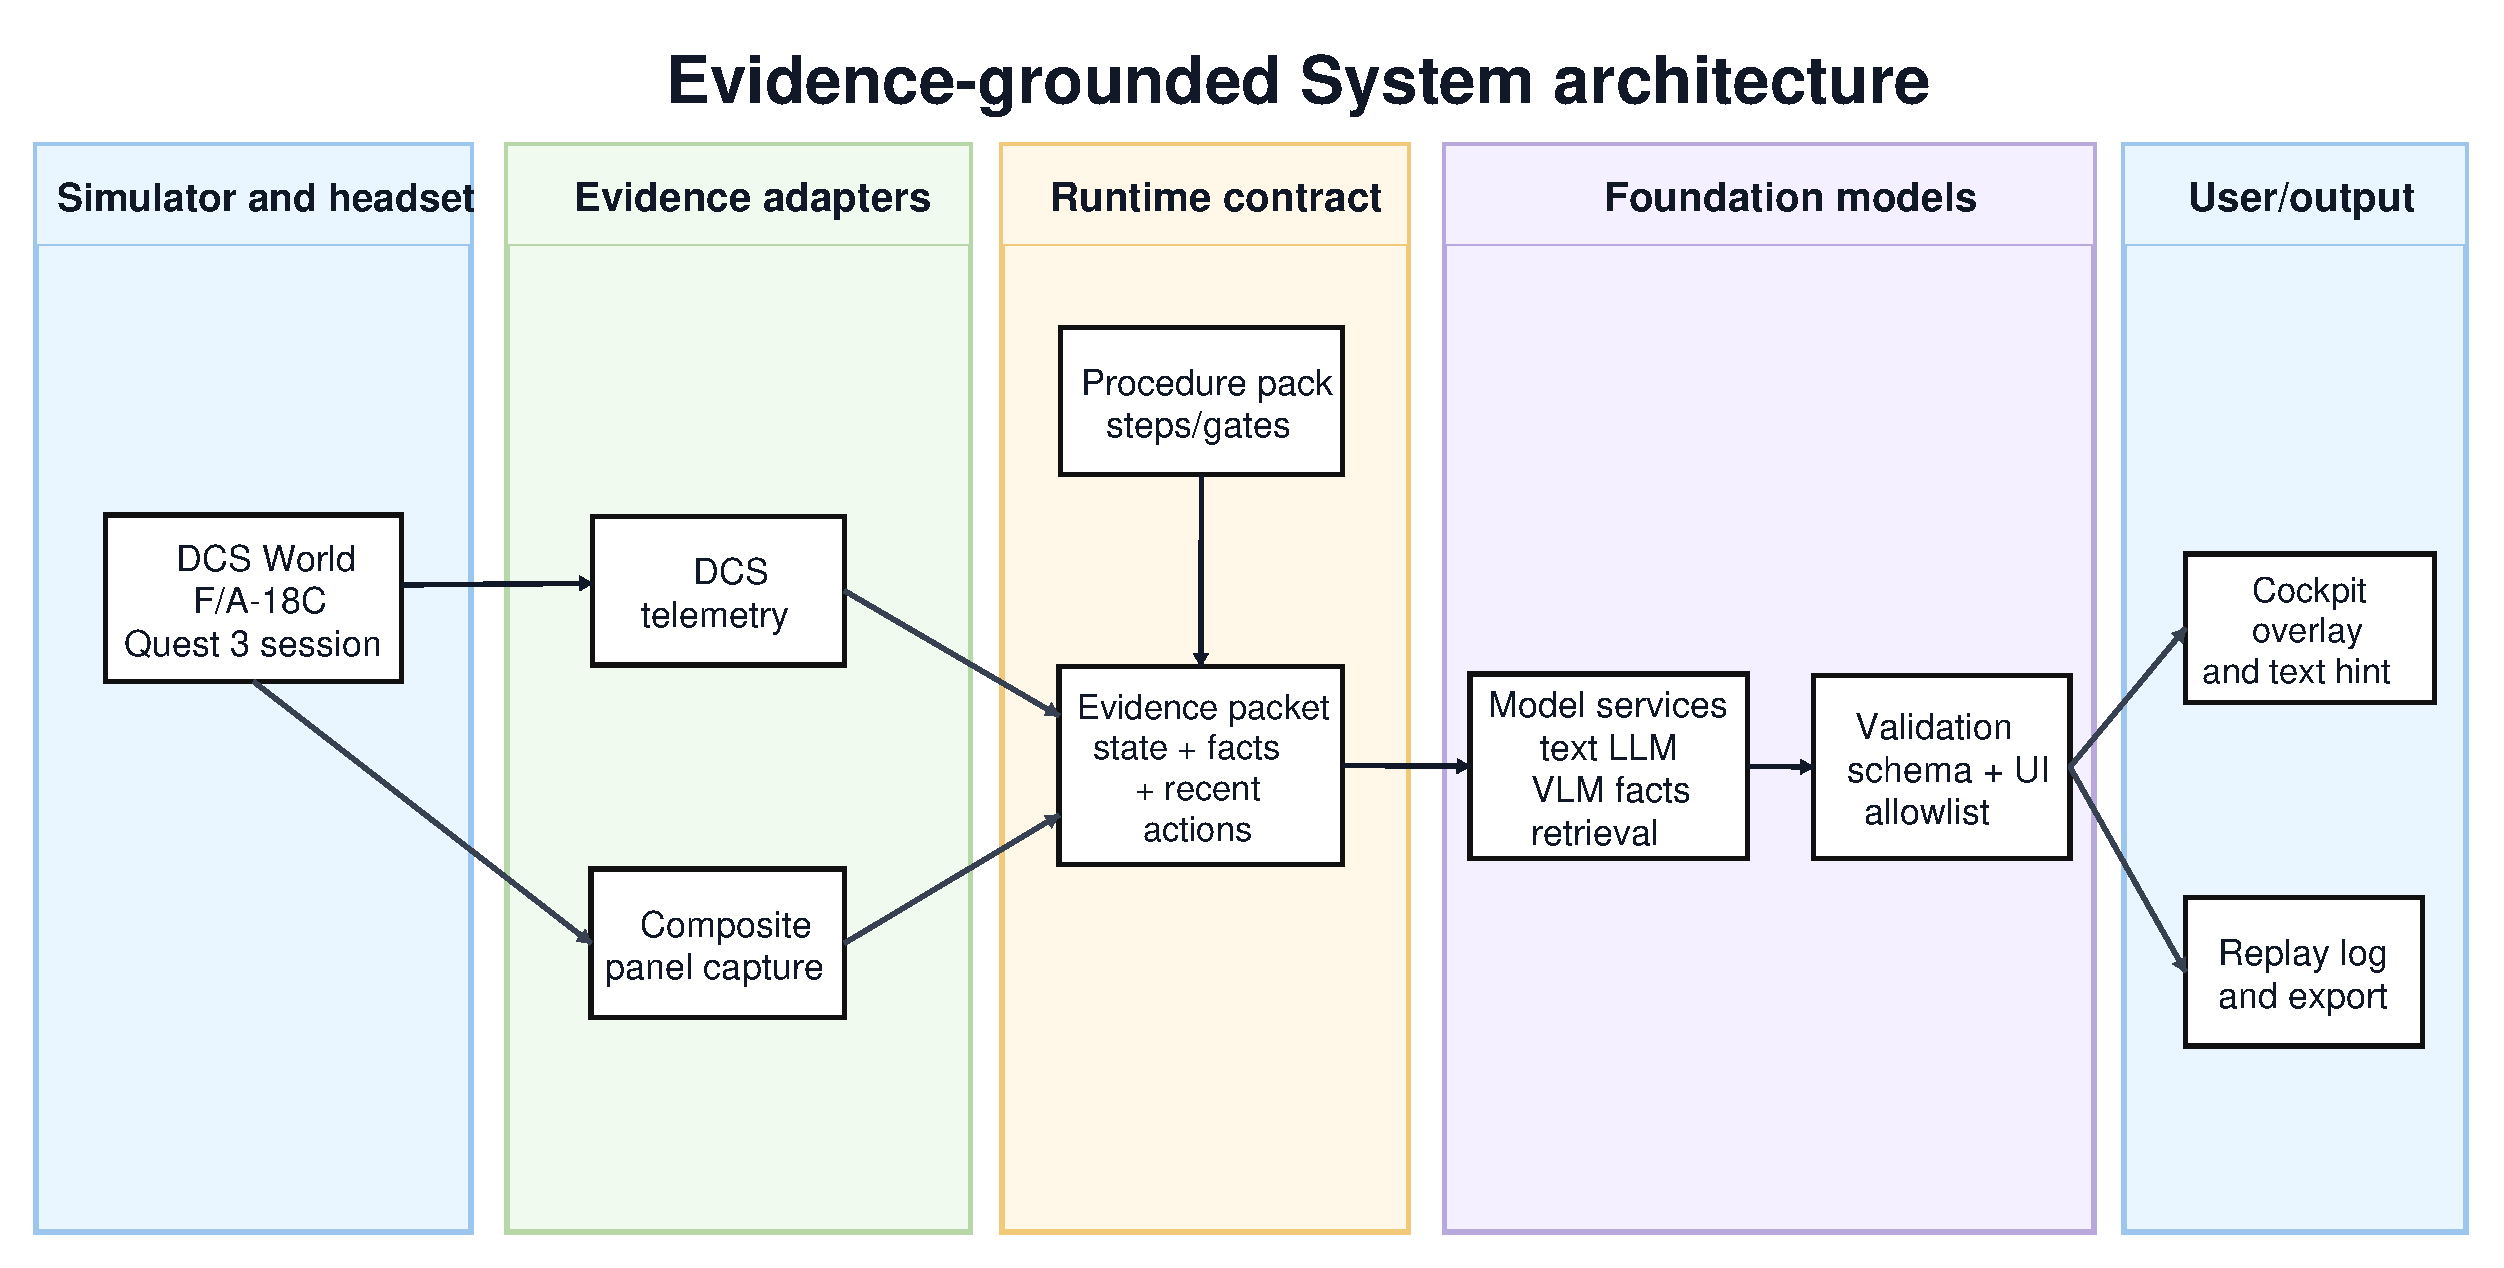
\includegraphics[width=\textwidth]{figures/fig_system_architecture.pdf}
  \caption[证据约束教学架构]{证据约束教学架构。模拟器遥测、复合面板视觉、过程包配置、检索到的知识以及模型输出通过证据包整合，并在覆盖层或教学文本到达座舱之前由校验器进行检查。}
  \label{fig:system-architecture}
\end{figure}

同样的边界也支持研究工作流程。关于门控、证据包、校验器决策和回放的技术声明可以使用fixture进行测试。关于视觉事实提取的声明可以与实时教学分开进行基准测评。关于VR呈现的声明可以作为形成性先导证据处理，而非验证架构的前提条件。

% ===========================================================================
\section{证据约束帮助循环}\label{sec:design-dataflow}

实时帮助循环是核心运行时的调用链。简洁地表示为：

\begin{center}
\small
帮助触发 $\rightarrow$ 遥测快照 $\rightarrow$ 可选视觉捕获 $\rightarrow$ 步骤与门控推断 $\rightarrow$ 证据包 $\rightarrow$ 检索 $\rightarrow$ 模型响应 $\rightarrow$ 校验器验证 $\rightarrow$ 覆盖层/文本输出 $\rightarrow$ 事件日志
\end{center}

这个顺序很重要，因为它确定了权威的来源顺序。模型并非首先决定模拟器状态意味着什么。相反，运行时在生成之前组装状态证据和候选步骤，并在显示之前验证生成的响应。图~\ref{fig:help-cycle}~展示了这一循环。

\begin{figure}[htbp]
  \centering
  
\includegraphics[width=\textwidth]{figures/fig_help_cycle.pdf}
  \caption{实时证据约束帮助循环。每一次帮助请求被转换为遥测和视觉观测，对照过程门控进行解释，通过检索到的知识进行锚定，经过文本LLM处理后由校验器验证，然后以覆盖层/文本输出形式分发，并附带事件日志追踪。}
  \label{fig:help-cycle}
\end{figure}

\subsection{帮助循环各阶段}

\textbf{观测 (Observation).}
DCS-BIOS适配器接收模拟器状态，遥测管线将其规范化为运行时变量。当活跃或可能活跃的步骤需要显示证据时，视觉适配器可以捕获复合座舱面板图像并请求视觉事实提取。

\textbf{候选推断 (Candidate inference).}
过程引擎评估前置条件和完成门控，识别候选步骤，并记录缺失或不确定的证据。生成的候选不是自然语言建议，而是从当前证据中推导出的结构化运行时对象。

\textbf{证据包组装 (Evidence packet assembly).}
运行时收集遥测值、门控结果、最近变化增量、视觉事实状态、检索到的来源引用以及步骤候选，组装为证据包。该证据包是状态解释与模型辅助帮助生成之间的边界对象。

\textbf{模型响应 (Model response).}
提示词要求模型基于证据包生成结构化的帮助响应。输出必须符合运行时HelpResponse Schema。无法解析或无法安全映射的自由文本不会成为可执行操作。

\textbf{验证与映射 (Validation and mapping).}
响应经过JSON提取、Schema验证、证据引用检查、步骤与目标白名单以及校验器验证。只有通过这些检查的响应才能映射为覆盖层操作或教学文本。验证失败会触发修复、拒绝或确定性回退。

\textbf{执行与日志 (Execution and logging).}
覆盖层命令仅限于安全的显示操作，如高亮、脉冲或清除。控制注入和自动点击不在架构范围内。每一次帮助循环均被记录为结构化事件，以便会话结束后可回放。

\subsection{Schema级别证据锚定}

证据锚定在输出执行之前强制执行。HelpResponse Schema根据当前过程包和UI映射生成，因此有效步骤和覆盖层目标的集合是任务特定的。模型提出的每个目标必须附带证据，其类型和引用必须与帮助循环上下文中可用的数据相对应。支持的证据类型包括遥测变量（\texttt{var}）、门控评估（\texttt{gate}）、检索到的来源（\texttt{rag}）、最近状态变化（\texttt{delta}）以及视觉事实（\texttt{visual}）。

这种设计改变了未经支持的模型响应的失败模式。如果模型提出了一个貌似合理但未经锚定的覆盖层操作，该响应不仅是作为可疑记录记入日志，而是在结构上对操作执行无效。系统随后可以修复到允许的目标、回退到纯文本引导，或拒绝该操作计划。

% ===========================================================================
\section{遥测作为状态证据}\label{sec:design-telemetry}

遥测是控制器、指示器和DCS-BIOS直接导出的数值状态值的主要证据来源。遥测管线通过四个阶段将原始模拟器帧转换为稳定的状态证据：

\begin{enumerate}
\item \textbf{原始摄入 (Raw ingestion).} DCS-BIOS UDP帧被解码为带有时间戳和序列信息的结构化观测。

\item \textbf{变量解析 (Variable resolution).} 过程包映射将原始BIOS字段投影到规范化变量上，例如 \texttt{rpm\_r}、\texttt{apu\_ready} 或 \texttt{battery\_on}。解析器同时追踪缺失的数据源，使运行时能够区分观测到的假值与不可用的值。

\item \textbf{增量清洗 (Delta sanitisation).} 配置的阈值、去抖窗口和过滤策略抑制由传感器抖动、开关弹跳和乱序帧引起的虚假变化。

\item \textbf{增量聚合 (Delta aggregation).} 最近的状态变化被压缩为适合提示词的摘要，并作为帮助循环推理的证据来源。
\end{enumerate}

缺失来源的区分对于过程性教学很重要。当开关已知为关闭状态与遥测来源缺失时，门控的失败方式不应相同。第一种情况可以证明纠正性引导是合理的；第二种情况可能需要带有不确定性或纯文本的帮助。

% ===========================================================================
\section{过程引擎与证据门控}\label{sec:design-procedure}

过程引擎维护有序冷启动序列的状态。每个步骤可以是待处理、活跃、已完成或阻塞状态，状态转移由前置条件和完成门控驱动。门控以声明式方式在过程包中表达，而非嵌入提示词中。这确保过程状态是由规则支配的领域决策，而非模型推断。

门控评估器支持阈值检查、范围检查、布尔标志和经过时间条件。缺失、来源缺失或哨兵值会产生诊断性失败，而非被静默地强制转换为有效状态。这些诊断信息同时反馈给证据包和确定性回退。

\subsection{确定性回退}

确定性回退是架构的一部分，而非事后的紧急补救措施。当模型不可用或模型输出验证失败时，运行时根据活跃步骤、未满足的门控、最近操作和证据可用性计算出保守的提示。它区分硬阻塞（证据显示某门控未满足）和软阻塞（所需证据缺失或不确定）。覆盖层输出被抑制，除非局部规则能够唯一确定一个有效目标。

\subsection{按证据来源进行步骤分类}

当前的F/A-18C过程包根据最可靠的可获得证据来源对步骤进行分类：

\begin{itemize}
\item \textbf{视觉优先步骤：} S08、S15、S18和S19需要来自视觉事实管线的座舱显示证据。
\item \textbf{BIOS优先步骤：} S01、S03--S13、S16和S20--S33在过程包元数据中声明为主要通过遥测验证。
\item \textbf{手动或面板外步骤：} S14和S17需要手动确认，或涉及三屏复合面板之外的座舱区域。
\end{itemize}

火警测试步骤S02通过其自身的门控和最近操作契约处理，而非通过过程包中的三个优先级列表。重要的架构要点是：运行时不会让模型来决定哪个证据通道对某个步骤具有权威性。该选择由过程包声明，并由帮助循环消费。

% ===========================================================================
\section{校验器工程与证据验证}\label{sec:design-harness}

校验器是输出到达模拟器之前的最终安全边界。它将模型提出的响应转换为经过验证的操作计划，或转换为修复、拒绝或纯文本结果。详细的对象关系见附录图~\ref{fig:harness-validation}；此处仅概述其主要的架构角色。

校验器使用四个概念对象：

\begin{description}
\item[\texttt{EvidencePacket}.]
当前帮助循环的规范化快照：遥测状态、门控诊断、最近操作、视觉事实、检索到的引用以及候选步骤信息。

\item[\texttt{StepCandidate}.]
关于学习者可能位于过程哪个位置的候选解释，由门控、遥测、最近操作和视觉证据推导得出。

\item[\texttt{StepHarnessSpec}.]
每个步骤的过程包派生契约：允许的覆盖层目标、所需的可观测项、遥测事实、视觉事实、完成谓词、恢复策略和信号新鲜度要求。

\item[\texttt{HarnessActionPlan}.]
验证后的结果：选中的步骤、选中的覆盖层步骤、目标、证据引用、引导文本、纯文本状态、修复状态、拒绝状态及原因。
\end{description}

验证序列具有三个效果。第一，它防止错误步骤或错误目标的输出绕过过程包。第二，它防止陈旧或不适当的证据驱动后续步骤。第三，它为修复和拒绝创建机器可读的原因，这些原因随后可用于回放和评估。

\subsection{基于Fixture的回归测试}

校验器通过实时帮助fixture进行测试：在曾经暴露失败的特定过程状态下记录的遥测快照和运行时上下文。每个fixture通过帮助循环回放，并断言期望的结果，例如正确的目标、修复后的目标、纯文本回退或安全拒绝。

当前的覆盖矩阵包含20个实时fixture回归条目，覆盖S01--S33。这些fixture涵盖正确推进、错误目标拒绝、不完整或不匹配视觉证据的修复、防止陈旧的VLM事实泄漏到非视觉步骤、移动控件等待引导，以及开关、按钮和旋转控件的交互语义。这一覆盖范围并非教育评估，而是技术证据，证明证据锚定约束可以在运行时边界上被系统性地执行。

% ===========================================================================
\section{适配器边界：模拟器、覆盖层与视觉}\label{sec:design-adapters}

适配器层将DCS特定行为隔离在核心层使用的端口之后。三个适配器职责对实时运行时至关重要。

\begin{description}
\item[遥测输入 (Telemetry input).]
遥测适配器接收DCS-BIOS状态数据并馈送给遥测管线。其输出是规范化的状态证据，而非模拟器特定的帧数据。

\item[覆盖层输出 (Overlay output).]
覆盖层适配器将抽象的教学目标映射为DCS覆盖层标识符，并发送高亮、脉冲或清除命令。它不执行座舱控制操作。

\item[视觉输入 (Vision input).]
视觉适配器触发截图捕获，并将复合面板图像传递给VLM事实提取器。生成的视觉事实作为结构化证据返回核心层。
\end{description}

VR路径遵循相同的边界。VR镜面显示、教学文本传输和复合面板捕获属于适配器的关注范围；过程推断和校验器验证保留在核心层。VR代码路径已在第~\ref{sec:eval-pilot}~节报告的形成性先导研究中得到使用。更大规模的受控人类受试者评估仍属未来工作。

% ===========================================================================
\section{事件日志与回放}\label{sec:design-replay}

可审计性要求帮助循环决策在实时会话结束后仍然可被追溯。运行时以JSONL格式记录版本化、带时间戳的事件。事件包括观测、帮助请求、证据摘要、模型输出、校验器决策、覆盖层操作以及与评分相关的交互数据。

回放使用这些记录离线重建步骤顺序、状态机一致性和帮助循环行为。当前的回放评估套件包括五种场景类型：无操作、接通电池、电池与发电机断开、FCS重置与BIT以及INS对准。这些案例使用DCS-BIOS原始捕获数据，并在可能的情况下使用视觉sidecar产物。

日志和回放层从两个方面支撑本论文。在开发过程中，它使回归可重现。在评估过程中，它将关于就绪性和仪表化的声明的论证基础连接到具体的产物，而非仅依赖人工观察。具有同步视觉帧的多模态人在回路会话的完整端到端回放目前仍是一个局限。

% ===========================================================================
\section{VLM视觉证据适配器}\label{sec:design-vlm}

VLM组件为遥测未直接导出的显示状态提供视觉证据。其运行时输出是一组视觉事实，而非过程决策。每个事实是关于可见座舱显示内容的有限命题，状态为 \texttt{seen}、\texttt{not\_seen} 或 \texttt{uncertain}。过程引擎和校验器决定这些事实如何影响帮助循环。

当前运行时契约使用第~\ref{ch:background}~章中介绍的本体，包含13个事实。事实具有生存时间（TTL）设置、可选的粘性语义，以及通过all-of或any-of条件的步骤绑定。例如，与FCS-MC最终GO相关的事实可以被锁存，以便学习者在切换页面时不会丢失已完成的瞬态显示状态。

当帮助请求涉及视觉优先步骤时，运行时可以触发截图捕获，提取视觉事实，将其合并到当前证据快照中，并纳入证据包。如果视觉适配器不可用或多模态请求失败，帮助循环将继续使用遥测、检索和过程门控。这种优雅降级保留了遥测锚定的核心功能，同时允许视觉证据改善需要显示内容解释的步骤。

数据管线、本体从8个事实到13个事实的演进、LoRA微调配置以及留出集基准测评协议属于方法论问题而非架构问题，因此安排在第~\ref{ch:methodology}~章讨论，并在第~\ref{ch:evaluation}~章进行评估。

% ===========================================================================
\section{本章小结}\label{sec:design-summary}

本章提出的架构将基础模型教学转变为受约束的证据处理管线。遥测和视觉事实提供观测数据，过程包定义有效的状态转移和证据需求，检索提供来源锚定的上下文，模型生成结构化的帮助，校验器验证或修复提出的操作，日志使决策可回放。这是从系统层面回答RQ1：当模型输出被置于显式证据的下游和强制验证的上游时，过程性帮助就变得可审计。
